\documentclass[../analysisII_notes.tex]{subfiles}
\begin{document}
\section{Aula 10 - 07 de Abril, 2025}
\subsection{Motivações}
\begin{itemize}
	\item Considerações Finais;
	\item Medida Nula.
\end{itemize}
\subsection{Considerações Finais - Parte 2.}
Conforme vimos na última aula, estávamos provando um teorema relacionado ao cálculo de integrais, mas ficou \hyperlink{next_class_11}{\textit{faltando provar um limite.}} Partiremos deste ponto:
\begin{proof*}[\hyperlink{next_class_11}{\textit{Continuação}}]
	Dado um valor c entre a e b, então pela aditividade, podemos escrever
	\[
		\int_{a}^{b}f = \int_{a}^{c}f + \int_{c}^{b}f \Longleftrightarrow \biggl\vert \int_{a}^{b}f - \int_{a}^{c}f \biggr\vert = \biggl\vert \int_{c}^{b}f \biggr\vert.
	\]
	Note que podemos aplicar a versão da desigualdade triangular observada anteriormente, tal que
	\[
		\biggl\vert \int_{a}^{b}f - \int_{a}^{c}f \biggr\vert = \biggl\vert \int_{c}^{b}f \biggr\vert \leq \int_{c}^{b}|f|.
	\]
	Sendo f limitada, existe um valor K positivo que limita seu módulo para qualquer valor em seu domínio; logo,
	\[
		\biggl\vert \int_{a}^{b}f - \int_{a}^{c}f \biggr\vert \leq \int_{c}^{b} |f| \leq \int_{c}^{b}K = K(b-c)
	\]
	e, passando o limite conforme c se aproxima de b pela esquerda, temos
	\[
		0\leq \lim_{c\to b^{-}}\biggl\vert \int_{a}^{b}f-\int_{a}^{c}f \biggr\vert \leq K (b-c) \overbracket[0pt]{\longrightarrow}^{c\to b^{-}}0. \text{ \qedsymbol}
	\]
\end{proof*}
\begin{tcolorbox}[
		skin=enhanced,
		title=Observação,
		fonttitle=\bfseries,
		colframe=black,
		colbacktitle=cyan!75!white,
		colback=cyan!15,
		colbacklower=black,
		coltitle=black,
		drop fuzzy shadow,
	]
	Analogamente a este teorema, se \(f:[a, b]\rightarrow \mathbb{R}\) for limitada e tal que, para todo número c, estritamente maior que a, entre a e b, a restrição de f \(f|_{[c, b]}\) for integrável, então a f em si também o é; além disso,
	\[
		\int_{a}^{b} f = \lim_{c\to a^{+}}\int_{c}^{b}f.
	\]

	Isso permite, por exemplo, integrar a função \(f:[0, 1]\rightarrow \mathbb{R}\) dada por
	\[
		f(x) = \left\{\begin{array}{ll}
			0,                                  & \quad x = 0       \\
			\sin^{}{\biggl(\frac{1}{x}\biggr)}, & \quad x\in (0, 1]
		\end{array}\right..
	\]
	Vemos que o valor de f(x) oscila entre -1 e 1, então ela é limitada; também, dado c no domínio de f, sua restrição \(f|_{[c, 1]}\) é contínua. No entanto, não existe o limite para de x convergindo diretamente ao 0 pela esquerda, então, à primeira vista, não conseguiríamos integrar essa função.

	O pulo do gato aqui é justamente que ela satisfaz o teorema, então, como sua restrição é contínua, essa restrição é integrável, donde a própria f é integrável em \([0, 1]\) e sua integral é calculável.
\end{tcolorbox}
\begin{exr}
	Prove o que foi afirmado na observação acima.
\end{exr}
\hypertarget{mean_value_theorem}{
	\begin{theorem*}[Teorema do Valor Médio para Integrais]
		Suponha que \(f:[a, b]\rightarrow \mathbb{R}\) é uma função contínua. Existe um valor no domínio de f cuja área retangular (da base b-a e altura f(c)) coincide com a integral da f neste intervalo: ou seja, tem pelo menos um c entre a e b tal que
		\[
			f(c) = \frac{1}{b-a}\int_{a}^{b}f(x)dx.
		\]
	\end{theorem*}
}
\begin{figure}[H]
	\begin{center}
		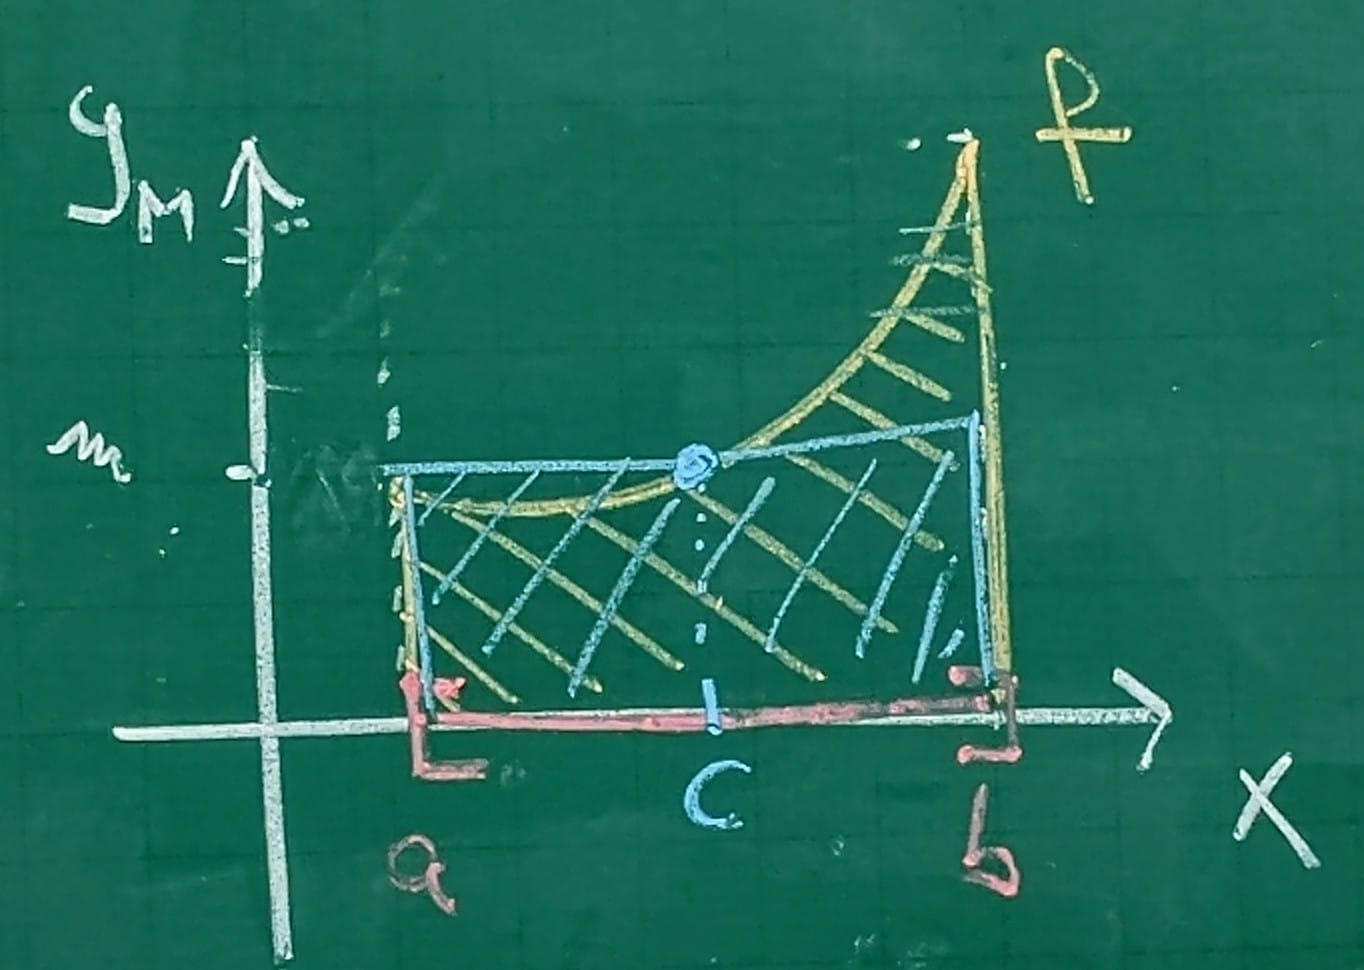
\includegraphics[height=0.5\textheight, width=0.5\textwidth, keepaspectratio]{./Images/mvt_integral_10.png}
	\end{center}
	\caption{em algum ponto dentro do intervalo, o retângulo azul coincide, em área, com a integral da função.}
	\label{mvt10}
\end{figure}
\begin{proof*}
	Com efeito, denotando os valores ínfimo e supremo de f por m e M respectivamente, temos
	\[
		m \leq f(x)\leq M \Rightarrow \int_{a}^{b}m \leq \int_{a}^{b}f \leq \int_{a}^{b} M \Rightarrow m(b-a) \leq \int_{a}^{b}f \leq M(b-a).
	\]
	Dividindo tudo por (b-a), a desigualdade mais à direita torna-se
	\[
		m \leq \frac{1}{b-a}\int_{a}^{b} f \leq M.
	\]
	Sendo f contínua, existem valores \(x_{1}\) e \(x_2\) em seu domínio onde f assume os valores de m e M, pelo \hyperlink{weierstrass_theorem}{\textit{teorema de Weierstrass}}. Logo,
	\[
		m = f(x_1) \leq \frac{1}{b-a}\int_{a}^{b}f \leq f(x_2) = M.
	\]
	Portanto, pelo \textit{teorema do valor intermediário }, existe ao menos um c no domínio de f tal que
	\[
		f(c) = \frac{1}{b-a}\int_{a}^{b}f.\quad \text{\qedsymbol}
	\]
\end{proof*}
\begin{theorem*}
	Se \(f:[a, b]\rightarrow \mathbb{R}\) é contínua e satisfaz:
	\begin{itemize}
		\item[i)] f é não-negativa:
		      \[
			      f(x)\geq 0, \quad \forall x\in [a, b];
		      \]
		\item[ii)] A integral de f é nula;
	\end{itemize}
	Nestas condições, f é a função nula, dada por
	\[
		f(x) = 0\; \forall x\in [a, b].
	\]
\end{theorem*}
\begin{proof*}
	A prova segue por contradição, então supomos que f não é a função nula. Consequentemente, existe pelo menos um ponto \(x_{0}\) no seu domínio onde ela não é 0. Pelo item i, então,
	\[
		f(x_{0}) > 0
	\]
	e, sendo contínua, ela também será positiva em uma vizinhança de \(x_{0}\) (um pequeno intervalo aberto \((x_{0}-\delta , x_{0}+\delta )\) em volta de \(x_{0}\)), o que significa que existem valores positivos \(\delta > 0\) e \(\alpha > 0\) tais que
	\[
		[x_{0}-\delta , x_{0}+\delta ]\subseteq [a, b] \quad\&\quad f(x)\geq \alpha,\; \forall x\in [x_{0}-\delta , x_{0}+\delta].
	\]

	\begin{figure}[H]
		\begin{center}
			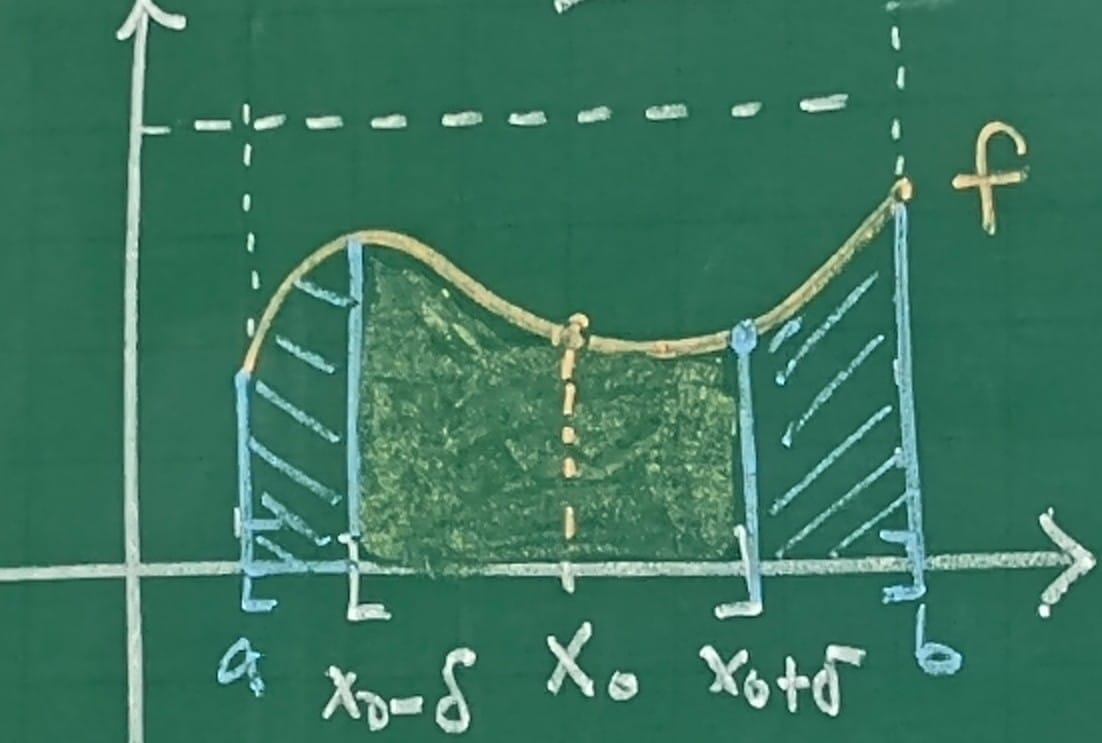
\includegraphics[height=0.5\textheight, width=0.5\textwidth, keepaspectratio]{./Images/neighborhood_10.png}
		\end{center}
		\caption{aditividade aplicada a uma pequena vizinhança em torno do ponto onde f não anula-se.}
		\label{nghbd10}
	\end{figure}
	Portanto, podemos escrever, com o \hyperlink{integral_additivity}{\textit{teorema da aditividade das integrais}},
	\[
		\int_{a}^{b} f = \int_{a}^{x_{0}-\delta }f + \int_{x_{0}-\delta }^{x_{0}+\delta }f + \int_{x_{0}+\delta }^{b}f \geq \int_{x_{0}-\delta }^{x_{0}+\delta }f\geq \int_{x_{0}-\delta }^{x_{0}+\delta } \alpha >0. \text{ \qedsymbol}
	\]
\end{proof*}
\begin{theorem*}
	Se \(f:[a, b]\rightarrow \mathbb{R}\) é limitada e possui apenas um número finito de descontinuidades, digamos, por exemplo, como o conjunto
	\[
		D = \{x_1 < x_2 < \dotsc < x_{n}\}\subseteq [a, b],
	\]
	então f é integrável.
\end{theorem*}
\begin{exr}
	Prova deixada como exercício.
\end{exr}

\begin{figure}[H]
	\begin{center}
		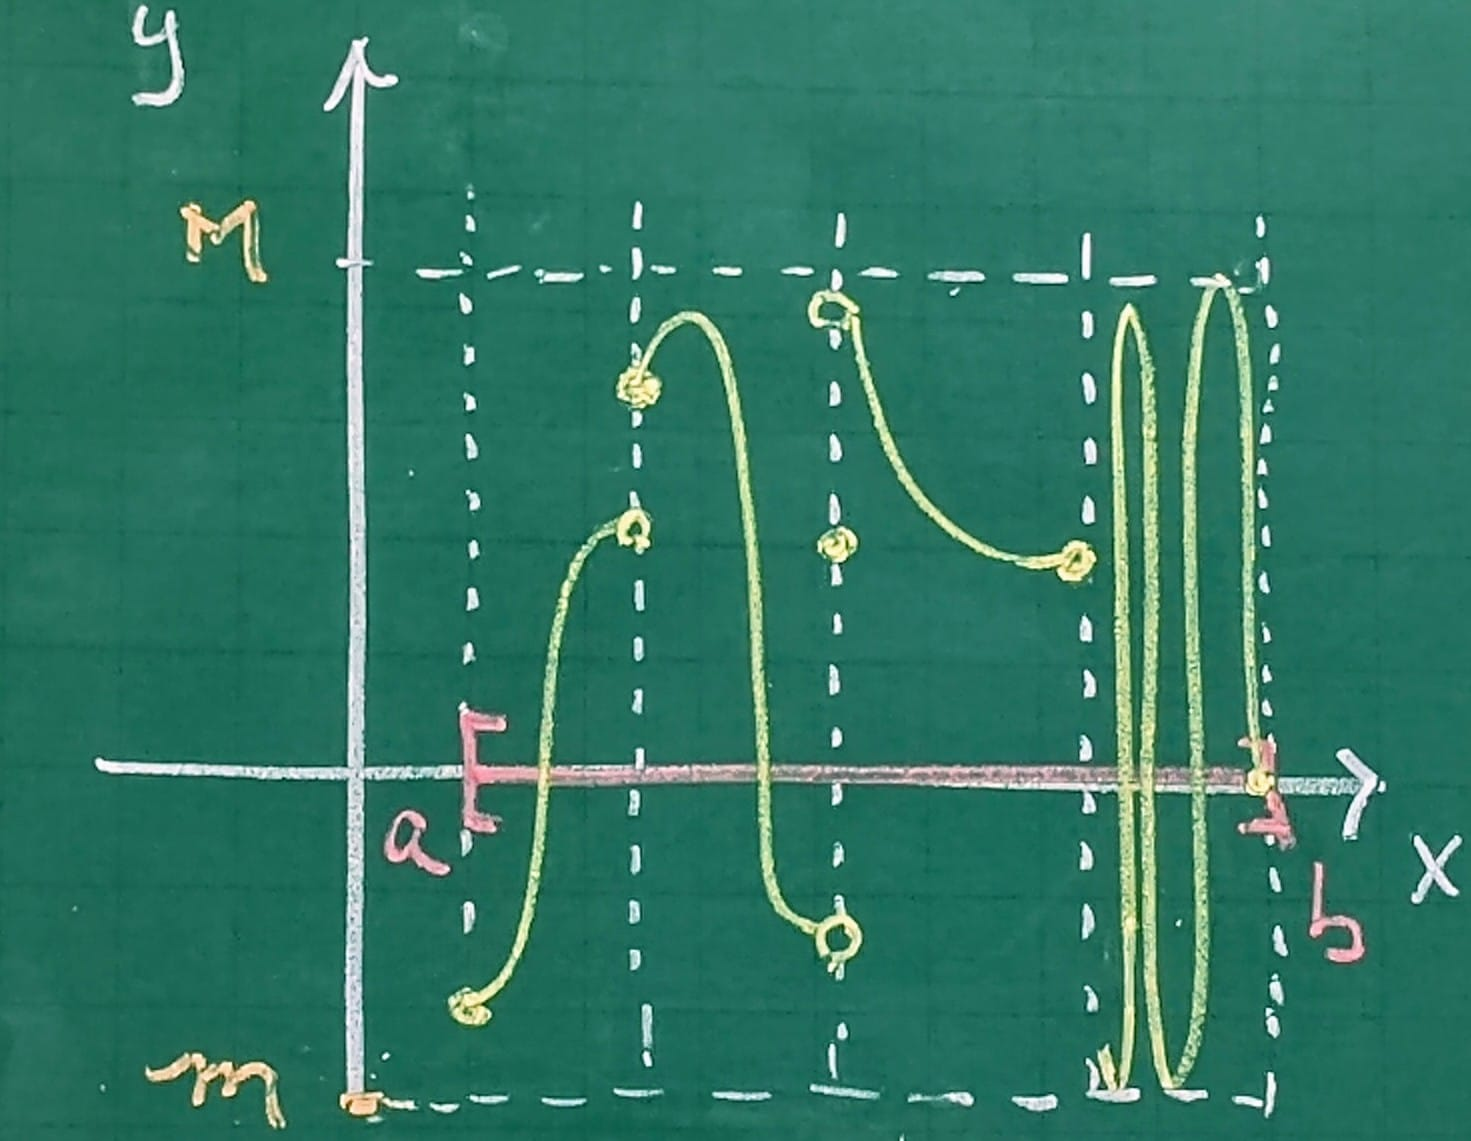
\includegraphics[height=0.5\textheight, width=0.5\textwidth, keepaspectratio]{./Images/discontinuity_10.png}
	\end{center}
	\caption{exemplo de função para o teorema.}
	\label{discontinuity10}
\end{figure}

Com isso, encerramos as considerações finais, e passamos a estudar a caracterização de Lebesgue das funções Riemann-Integráveis.

\subsection{Caracterização de Lebesgue das Funções Riemann-Integráveis.}
Começamos esta parte fixando a seguinte notação: se I for um intervalo contido na reta real com extremos \(a < b\), seu comprimento será denotado por
\[
	\ell (I) \coloneqq b-a.
\]
Com essa notação,
\[
	\ell ([a, b]) = \ell ((a, b)) = \ell ((a, b]) = \ell ([a, b)) = b-a.
\]
\begin{def*}
	Um subconjunto E da reta real possui \textbf{medida nula}, ou \textbf{é um conjunto de medida nula}, denotado por \(m(E)=0\), quando, dado \(\varepsilon > 0\), existe uma sequência de intervalos abertos ou fechados
	\[
		I_1, I_2, \dotsc , I_{n}, \dotsc
	\]
	tais que:
	\begin{itemize}
		\item[I)] A união dos intervalos contém o conjunto E - os intervalos \textit{cobrem enumeravelmente} o E:
		      \[
			      E\subseteq \bigcup_{j=1}^{\infty}I_{j};
		      \]
		\item[II)] A soma dos comprimentos de todos os intervalos não excede \textit{nenhum} dos \(\varepsilon \)'s:
		      \[
			      \sum\limits_{j=1}^{\infty}\ell (I_{j}) <\varepsilon .\quad \square
		      \]
	\end{itemize}
\end{def*}

A propriedade (II) garante que podemos deixar o tamanho total do intervalo cobrindo \(E\) o quão pequeno queiramos.
\begin{prop*}[Propriedades dos Conjuntos de Medida Nula]
	\begin{itemize}
		\item[i)] Um conjunto com único ponto é de medida nula:
		      \[
			      m(\{a\}) = 0,\; \forall a\in \mathbb{R};
		      \]
		\item[ii)] Se A e B são subconjuntos da reta real, com A sendo subconjunto de B, então
		      \[
			      m(B) = 0 \Rightarrow m(A) = 0,
		      \]
		      ou seja, um conjunto de medida nula não pode conter um conjunto sem medida nula;
		\item[iii)] Se \((E_{i})_{i\in \mathbb{N}}\) for uma sequência de conjuntos, todos de medida nula, então
		      \[
			      m \biggl(\bigcup_{i=1}^{\infty}E_{i}\biggr) = 0;
		      \]
		\item[iv)] Qualquer intervalo \([a, b]\), com \(a < b\), \textbf{não} tem medida nula.
	\end{itemize}
\end{prop*}
\end{document}
